\documentclass[compress]{beamer}
\usepackage{ifthen,verbatim}

\newcommand{\isnote}{}
\xdefinecolor{lightyellow}{rgb}{1.,1.,0.25}
\xdefinecolor{darkblue}{rgb}{0.1,0.1,0.7}
\xdefinecolor{darkgray}{rgb}{0.3,0.3,0.3}

%% Uncomment this to get annotations
%% \def\notes{\addtocounter{page}{-1}
%%            \renewcommand{\isnote}{*}
%% 	   \beamertemplateshadingbackground{lightyellow}{white}
%%            \begin{frame}
%%            \frametitle{Notes for the previous page (page \insertpagenumber)}
%%            \itemize}
%% \def\endnotes{\enditemize
%% 	      \end{frame}
%%               \beamertemplateshadingbackground{white}{white}
%%               \renewcommand{\isnote}{}}

%% Uncomment this to not get annotations
\def\notes{\comment}
\def\endnotes{\endcomment}

\setbeamertemplate{navigation symbols}{}
\setbeamertemplate{headline}{\mbox{ } \hfill
\begin{minipage}{5.5 cm}
\vspace{-0.75 cm} \small
\end{minipage} \hfill
\begin{minipage}{4.5 cm}
\vspace{-0.75 cm} \small
\begin{flushright}
\ifthenelse{\equal{\insertpagenumber}{1}}{}{Jim Pivarski \hspace{0.2 cm} \insertpagenumber\isnote/\pageref{numpages}}
\end{flushright}
\end{minipage}\mbox{\hspace{0.2 cm}}\includegraphics[height=1 cm]{../cmslogo} \hspace{0.1 cm} \includegraphics[height=1 cm]{../tamulogo} \hspace{0.01 cm} \vspace{-1.05 cm}}

\newcommand{\s}[1]{{\mbox{\scriptsize #1}}}

\begin{document}
\begin{frame}
\vfill
\begin{center}
\textcolor{darkblue}{\Large Alignment of each endcap using beam-halo muons}

\vfill
\begin{columns}
\column{0.3\linewidth}
\begin{center}
\large
Jim Pivarski
\end{center}
\end{columns}

\begin{columns}
\column{0.3\linewidth}
\begin{center}
\scriptsize
{\it Texas A\&M University}
\end{center}
\end{columns}

\vfill
 8 October, 2010

\end{center}
\end{frame}

%% \begin{notes}
%% \item This is the annotated version of my talk.
%% \item If you want the version that I am presenting, download the one
%% labeled ``slides'' on Indico (or just ignore these yellow pages).
%% \item The annotated version is provided for extra detail and a written
%% record of comments that I intend to make orally.
%% \item Yellow notes refer to the content on the {\it previous} page.
%% \item All other slides are identical for the two versions.
%% \end{notes}

\small

%% \begin{frame}
%% % \frametitle{}
%% \begin{itemize}\setlength{\itemsep}{0.75 cm}
%% \item 
%% \end{itemize}
%% %% \hspace{-0.83 cm} \textcolor{darkblue}{\Large Outline2}
%% \end{frame}

\begin{frame}
\frametitle{Overview}
This is a long story involving two new alignment techniques.  Here it
is in reverse order:
\begin{enumerate}
\setcounter{enumi}{3}
\item To investigate possible barrel twist by anchoring transfer lines
  to multiple disks in each endcap\ldots

\setcounter{enumi}{2}
\item I have produced an alignment of each endcap from beam-halo
  tracks, rather than tracks from the tracker (also a good cross-check
  for Vadim)

\setcounter{enumi}{1}
\item To get sensible extrapolations of segments from one station to
  the next, we need to know the $\phi_y$ angles of the chambers\ldots

\setcounter{enumi}{0}
\item So I first aligned {\it only the $\phi_y$ angles} using
  collisions-TrackerMuons from the tracker.
\end{enumerate}

\vfill
The pre-alignment from the tracker \textcolor{darkblue}{(1)} is not introducing a twist into the
endcap because ``twist'' is $\phi_z$ vs.\ $z$, not $\phi_y$.

\vfill
\end{frame}

\begin{frame}
\frametitle{Classes of alignment parameters}

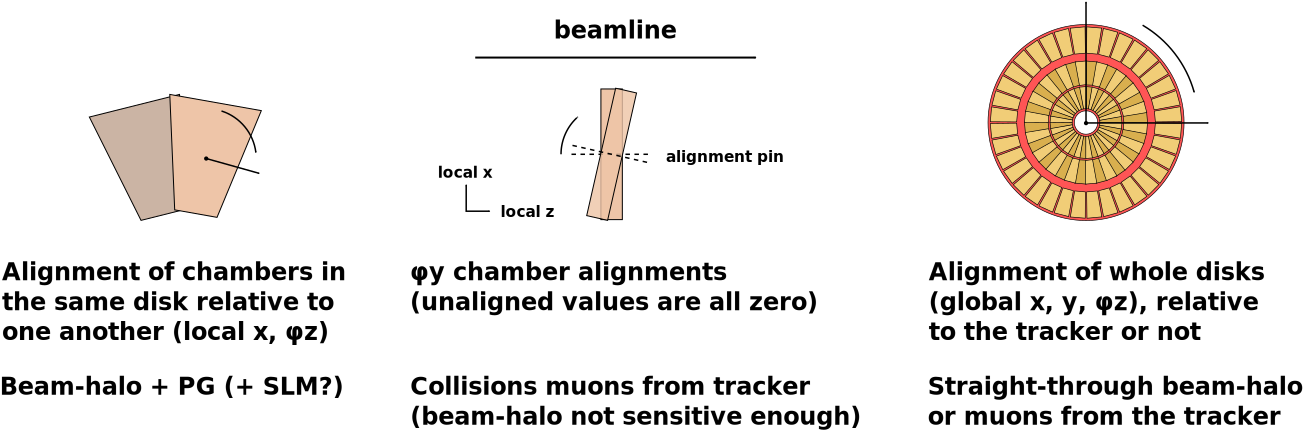
\includegraphics[width=\linewidth]{types_of_alignment.pdf}

\begin{itemize}
\item ($x$, $r\phi$) can be considered separate from $\phi_y$, though
  both can affect some types of residuals (making it difficult to
  determine how much of a residuals bias is local $x$ and how much is $\phi_y$)

\item Disk-scale alignment can be considered separate from
  individual- chamber alignment, though both affect muons from the
  tracker

\item The logical flow of solving the dependencies goes left-to-right,
  and the first step (chamber alignment from beam-halo) is already done
\end{itemize}
\end{frame}

\begin{frame}
\frametitle{History of $\phi_y$ alignments}

\vspace{0.1 cm}
\begin{columns}
\column{0.4\linewidth}
\includegraphics[width=\linewidth]{track_lhc_plane_closeup.png}

\column{0.6\linewidth}
\begin{itemize}
\item $\phi_y$ was the first parameter we attempted to measure with
  beam-halo, by assuming that straight muon tracks originate somewhere
  along an infinitely long, straight LHC beampipe

\item These assumptions are too strong, and the method doesn't work
  with $\vec{B} \ne 0$
\end{itemize}
\end{columns}

\hfill \includegraphics[height=3 cm]{overlaps.png}

\vspace{-3 cm}
\begin{itemize}
\item $\phi_y$ can in principle be measured with beam-halo
  \\ overlaps, but the resolution is poor (determined \\ from the width
  of the corresponding residuals \\ distribution)

\item $\phi_y$ was fixed to zero in the 2010 beam-halo alignment

\item Measuring $\phi_y$ with collisions muons from the tracker is
  completely straight-forward: just look for an angular difference
  between propagated muon and segment

\item Analysis with 2.9~pb$^{-1}$ of $|\vec{p}| > 30$~GeV/$c$
  TrackerMuons; \underline{\it $\phi_y$ only}
\end{itemize}

% 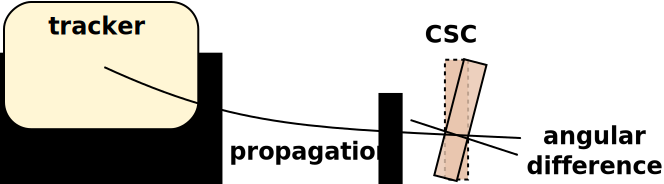
\includegraphics[width=\linewidth]{phiy_alignment.pdf}
\end{frame}

\begin{frame}
\frametitle{$\phi_y$ alignment results (example)}
\framesubtitle{See backup slides for complete results}
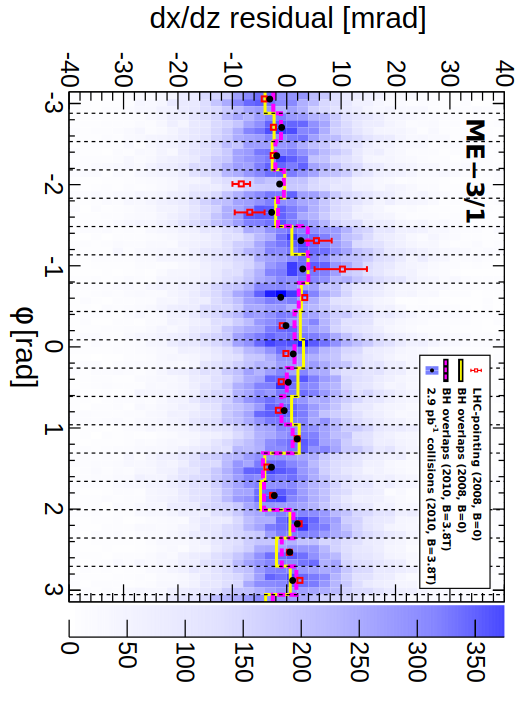
\includegraphics[height=\linewidth, angle=90]{mem3phiy_all.pdf}
\label{mem31phiy}
\end{frame}

\begin{frame}
\frametitle{Disk alignment with beam-halo}

\vspace{-0.3 cm}
\hfill \includegraphics[height=3 cm]{overlaps_straight_through.png}

\vspace{-3.5 cm}
\begin{itemize}
\item Beam-halo overlaps can \\ only align chambers within \\ the same ring
  to one another

\item Straight-through tracks \\ can align disks to one \\ another in the
  same endcap, \\ but resolution is smeared by \\ transit through the steel yoke

\item It will be essential to select high-momentum beam-halo muons

\item Though beam-halo is parallel to the axial field, it is
  influenced by the radial component of the magnetic field, which is
  large in the endcaps

\hfill \includegraphics[height=3 cm]{trackfit_resolution.pdf}
\hspace{0.1 cm} \includegraphics[height=3 cm]{trackfit_turnon.pdf}

\vspace{-3.3 cm}
\item MC study of \\ track-fit's \\ discriminating \\ power:
\end{itemize}
\end{frame}

\begin{frame}
\frametitle{Track-fit alternative}

\begin{itemize}
\item The momentum measurement from the standard track-fit depends
  on the positions of the disks, which is exactly what we want to
  align
\item To avoid a circular dependence, we can take advantage of the
  fact that muon chambers measure position and direction:
\begin{itemize}
\item measure momentum with the change in direction
\item align the positions
\end{itemize}
\end{itemize}
\begin{center}
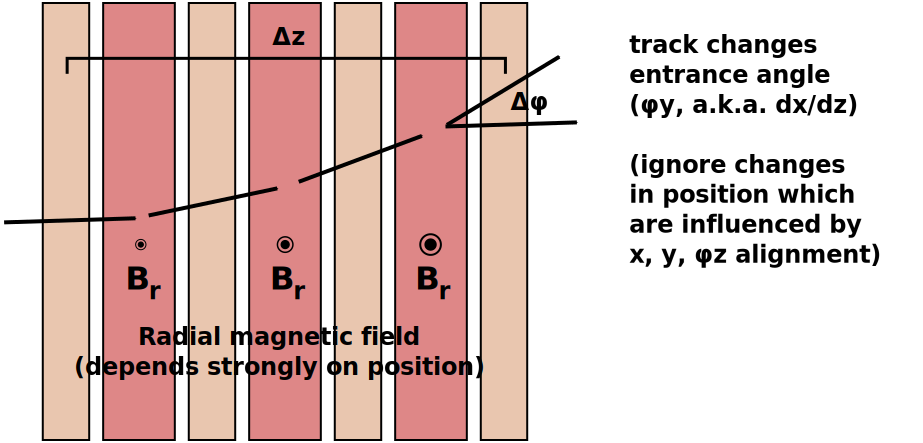
\includegraphics[width=0.85\linewidth]{pzfit.pdf}
\end{center}
\end{frame}

\begin{frame}
\frametitle{Track-fit alternative {\small (MC performance)}}

$p_z$ estimated from ME1, 2, 3:

\includegraphics[width=0.33\linewidth]{estimator123_resolution.pdf}
\includegraphics[width=0.33\linewidth]{estimator123_turnon.pdf}
\includegraphics[width=0.33\linewidth]{estimator123_occupancy.pdf}

\vfill
$p_z$ estimated from ME1, 2, 3, and 4:

\includegraphics[width=0.33\linewidth]{estimator1234_resolution.pdf}
\includegraphics[width=0.33\linewidth]{estimator1234_turnon.pdf}
\includegraphics[width=0.33\linewidth]{estimator1234_occupancy.pdf}

\vfill
We'll cut at 50~GeV/$c$, using the 4-station estimate only when
aligning ME4/1 and 4/2
\end{frame}

\begin{frame}
\frametitle{Beam-halo datasets}

\begin{columns}
\column{0.5\linewidth}
\centering LHC Tertiary Collimator Triplet test (Mar 10, 2010: 130434
and 130445)

\includegraphics[height=\linewidth, angle=90]{qpz_spectrum_TST.pdf}

\column{0.5\linewidth}
\centering Beam-halo collected during collisions \mbox{(Jun 10--Sep 1, 2010: 137437--144431)\hspace{-0.1 cm}}

\includegraphics[height=\linewidth, angle=90]{qpz_spectrum.pdf}
\end{columns}

\begin{itemize}
\item All plots of TCT and during-collisions look consistent, though
  during-collisions has an order of magnitude more data (important
  when applying a tight momentum cut)
\end{itemize}

(Note that tracks have ``CZ'' symmetry: we can't tell a westward-bound
muon from an eastern-bound antimuon)
\end{frame}

\begin{frame}
\frametitle{Beam-halo disk alignment}

\begin{itemize}
\item After applying high momentum cut (nearly parallel segments),
  linearly extrapolate segment from one disk to another and \\ compare
  position ($r\phi$ residual)

\item Residuals depend linearly on $1/(q\times p_z)$ because we're not
  taking track-curvature into account: linearly fit to get
  infinite-momentum limit in each $\phi$ bin

\item \only<1>{This is an example from ME$+$2 $\to$ ME$+$1/1 (strong $\vec{B}$-field)}\only<2>{This is an example from ME$+$3 $\to$ ME$+$4 (weak $\vec{B}$-field)}\only<3>{\mbox{This is an example from ME$+$2 $\to$ ME$+$3: same disk, should be zero\hspace{-1 cm}}}

(see backup for all plots)
\end{itemize}

\vfill
\begin{columns}
\column{0.33\linewidth}
\centering linear dependence on $1/(q\times p_z)$

\only<1>{\includegraphics[height=\linewidth, angle=90]{linear_mep2to1inner.pdf}}\only<2>{\includegraphics[height=\linewidth, angle=90]{linear_mep3to4.pdf}}\only<3>{\includegraphics[height=\linewidth, angle=90]{linear_mep2to3.pdf}}

\column{0.33\linewidth}
\centering $c_0 + c_1\sin\phi + c_2\cos\phi$ before alignment

\only<1>{\includegraphics[height=\linewidth, angle=90]{diskiter01_p2to1inner.pdf}}\only<2>{\includegraphics[height=\linewidth, angle=90]{diskiter01_p3to4.pdf}}\only<3>{\includegraphics[height=\linewidth, angle=90]{diskiter01_p2to3.pdf}}

\column{0.33\linewidth}
\centering \only<1-2>{flat distribution after alignment}\only<3>{same distribution; \\ not aligned}

\only<1>{\includegraphics[height=\linewidth, angle=90]{diskiter02_p2to1inner.pdf}}\only<2>{\includegraphics[height=\linewidth, angle=90]{diskiter02_p3to4.pdf}}\only<3>{\includegraphics[height=\linewidth, angle=90]{diskiter02_p2to3.pdf}}
\end{columns}

Note: color scale (number of hits) is logarithmic
\end{frame}

\begin{frame}
\frametitle{Importance of $\phi_y$ pre-alignment}

\begin{itemize}
\item Extrapolations from one disk to the next have a rather large
  lever arm; getting the initial chamber orientation wrong by 1~mrad
  means $>$1~mm errors in the next disk (more than 1~meter
  apart)

\item Discontinuities in the residuals imply a chamber-by-chamber error

\item Remember that $\phi_y$ was aligned using a different method
  (tracker-to-muon chambers) on different muons (from collisions)
\end{itemize}

\begin{columns}
\column{0.5\linewidth}
\centering ME$+$2 $\to$ $+$3 without $\phi_y$ alignments

\includegraphics[height=\linewidth, angle=90]{diskiter02_phiyzero_p2to3.pdf}

\column{0.5\linewidth}
\centering ME$+$2 $\to$ $+$3 with $\phi_y$ alignments

\includegraphics[height=\linewidth, angle=90]{diskiter02_p2to3.pdf}
\end{columns}
\end{frame}

\begin{frame}
\frametitle{Disk alignment results}

Corrections (relative to ideal) from beam-halo collected during collisions

\begin{tabular}{l c c c}
 & $x$ (mm) & $y$ (mm) & $\phi_z$ (mrad) \\\hline
ME$+$1/1 & $3.933 \pm 0.080$ & $-1.242 \pm 0.052$ & $-0.411 \pm 0.023$ \\
ME$+$1/2 & $3.564 \pm 0.105$ & $-0.727 \pm 0.081$ & $0.408 \pm 0.020$ \\
check $+$2 $\to$ $+$3 & $0.085 \pm 0.035$ & $0.837 \pm 0.024$ & $-0.085 \pm 0.009$ \\
ME$+$4/1 & $1.196 \pm 0.038$ & $4.838 \pm 0.028$ & $-0.474 \pm 0.010$ \\\hline
ME$-$1/1 & $-1.701 \pm 0.079$ & $-1.787 \pm 0.052$ & $-0.797 \pm 0.023$ \\
ME$-$1/2 & $-0.395 \pm 0.108$ & $-0.787 \pm 0.086$ & $-0.675 \pm 0.020$ \\
check $-$2 $\to$ $-$3 & $0.178 \pm 0.035$ & $-0.379 \pm 0.025$ & $-0.037 \pm 0.009$ \\
ME$-$4/1 & $-2.117 \pm 0.038$ & $0.230 \pm 0.027$ & $-0.449 \pm 0.010$ \\\hline
\end{tabular}

\textcolor{darkgray}{\begin{tabular}{l c c c}
Same for TCT & $x$ (mm) & $y$ (mm) & $\phi_z$ (mrad) \\\hline
ME$+$1/1 & $3.568 \pm 0.278$ & $-0.293 \pm 0.241$ & $-0.496 \pm 0.095$ \\
ME$+$1/2 & $3.824 \pm 0.343$ & $-0.580 \pm 0.341$ & $0.378 \pm 0.076$ \\
check $+$2 $\to$ $+$3 & $-0.353 \pm 0.109$ & $1.097 \pm 0.112$ & $-0.054 \pm 0.037$ \\
ME$+$4/1 & $0.752 \pm 0.102$ & $4.939 \pm 0.098$ & $-0.473 \pm 0.031$ \\\hline
ME$-$1/1 & $0.161 \pm 0.366$ & $-1.555 \pm 0.303$ & $-0.148 \pm 0.122$ \\
ME$-$1/2 & $-0.325 \pm 0.876$ & $-0.743 \pm 0.557$ & $-1.038 \pm 0.197$ \\
check $-$2 $\to$ $-$3 & $-0.135 \pm 0.162$ & $-0.792 \pm 0.137$ & $0.111 \pm 0.048$ \\
ME$-$4/1 & $-2.399 \pm 0.138$ & $0.119 \pm 0.114$ & $-0.402 \pm 0.038$ \\\hline
\end{tabular}}
\end{frame}

% \[ q \times p_z = \frac{B_r}{330\mbox{ cm T/GeV}} \, \frac{\Delta z}{\Delta \phi} \]

\begin{frame}
\frametitle{Conclusions}
\begin{itemize}
\item Two new measurements for endcap alignment:
\begin{itemize}
\item $\phi_y$ of chambers (which had to wait for collisions, but interestingly enough agrees with the ``LHC pointing'' method that required so many assumptions)
\item global $x$, $y$, $\phi_z$ of disks, {\it independently} of the standard tracker-to-muon chamber method
\end{itemize}

\item This will provide a cross-check for the standard procedure, but
  also gives us two aligned endcaps for anchoring
  transfer lines, to check for a barrel twist
\begin{itemize}
\item remember that the position of one endcap relative to the other
  is not constrained, nor is either endcap relative to the tracker
\item location of constants: {\tt \scriptsize /afs/cern.ch/user/p/pivarski/public/}

{\tt \scriptsize OCT7\_CSC\_beamhalo-PG-collisionsphiy-straightthrough-diskXYphiZ.db}
\end{itemize}
\end{itemize}

\label{numpages}
\end{frame}

%% \section*{First section}
\begin{frame}
\begin{center}
\Huge \textcolor{blue}{BACKUP}

\normalsize
\vspace{1 cm}
\begin{minipage}{0.7\linewidth}
\begin{itemize}
\item $\phi_y$ alignment plots
\item beam-halo disk alignment plots
\end{itemize}
\end{minipage}
\end{center}
\end{frame}

\begin{frame}
\frametitle{All of the $\phi_y$ alignment results}
\begin{center}
ME$+$1/1 (a and b)
\end{center}

\begin{columns}
\column{0.5\linewidth}
\centering Before

\includegraphics[height=\linewidth, angle=90]{iter01_mep11.pdf}

\column{0.5\linewidth}
\centering After (1 iteration)

\includegraphics[height=\linewidth, angle=90]{iter02_mep11.pdf}
\end{columns}

\begin{itemize}
\item Blue background is the $dx/dz$ residuals distribution
  vs.\ $\phi$ from TrackerMuons; dashed lines are the chamber boundaries
\item Black points are the actual corrections (zero if fewer than 30
  hits or uncertainty is larger than 3~mrad), derived from a Gaussian
  fit from $-2\times$RMS to $2\times$RMS
\end{itemize}
\end{frame}

\begin{frame}
\frametitle{All of the $\phi_y$ alignment results}
\begin{center}
ME$+$1/2
\end{center}

\begin{columns}
\column{0.5\linewidth}
\centering Before

\includegraphics[height=\linewidth, angle=90]{iter01_mep12.pdf}

\column{0.5\linewidth}
\centering After (1 iteration)

\includegraphics[height=\linewidth, angle=90]{iter02_mep12.pdf}
\end{columns}

\begin{itemize}
\item Blue background is the $dx/dz$ residuals distribution
  vs.\ $\phi$ from TrackerMuons; dashed lines are the chamber boundaries
\item Black points are the actual corrections (zero if fewer than 30
  hits or uncertainty is larger than 3~mrad), derived from a Gaussian
  fit from $-2\times$RMS to $2\times$RMS
\end{itemize}
\end{frame}
\begin{frame}
\frametitle{All of the $\phi_y$ alignment results}
\begin{center}
ME$+$1/3
\end{center}

\begin{columns}
\column{0.5\linewidth}
\centering Before

\includegraphics[height=\linewidth, angle=90]{iter01_mep13.pdf}

\column{0.5\linewidth}
\centering After (1 iteration)

\includegraphics[height=\linewidth, angle=90]{iter02_mep13.pdf}
\end{columns}

\begin{itemize}
\item Blue background is the $dx/dz$ residuals distribution
  vs.\ $\phi$ from TrackerMuons; dashed lines are the chamber boundaries
\item Black points are the actual corrections (zero if fewer than 30
  hits or uncertainty is larger than 3~mrad), derived from a Gaussian
  fit from $-2\times$RMS to $2\times$RMS
\end{itemize}
\end{frame}

\begin{frame}
\frametitle{All of the $\phi_y$ alignment results}
\begin{center}
ME$+$2/1
\end{center}

\begin{columns}
\column{0.5\linewidth}
\centering Before

\includegraphics[height=\linewidth, angle=90]{iter01_mep21.pdf}

\column{0.5\linewidth}
\centering After (1 iteration)

\includegraphics[height=\linewidth, angle=90]{iter02_mep21.pdf}
\end{columns}

\begin{itemize}
\item Blue background is the $dx/dz$ residuals distribution
  vs.\ $\phi$ from TrackerMuons; dashed lines are the chamber boundaries
\item Black points are the actual corrections (zero if fewer than 30
  hits or uncertainty is larger than 3~mrad), derived from a Gaussian
  fit from $-2\times$RMS to $2\times$RMS
\end{itemize}
\end{frame}

\begin{frame}
\frametitle{All of the $\phi_y$ alignment results}
\begin{center}
ME$+$2/2
\end{center}

\begin{columns}
\column{0.5\linewidth}
\centering Before

\includegraphics[height=\linewidth, angle=90]{iter01_mep22.pdf}

\column{0.5\linewidth}
\centering After (1 iteration)

\includegraphics[height=\linewidth, angle=90]{iter02_mep22.pdf}
\end{columns}

\begin{itemize}
\item Blue background is the $dx/dz$ residuals distribution
  vs.\ $\phi$ from TrackerMuons; dashed lines are the chamber boundaries
\item Black points are the actual corrections (zero if fewer than 30
  hits or uncertainty is larger than 3~mrad), derived from a Gaussian
  fit from $-2\times$RMS to $2\times$RMS
\end{itemize}
\end{frame}

\begin{frame}
\frametitle{All of the $\phi_y$ alignment results}
\begin{center}
ME$+$3/1
\end{center}

\begin{columns}
\column{0.5\linewidth}
\centering Before

\includegraphics[height=\linewidth, angle=90]{iter01_mep31.pdf}

\column{0.5\linewidth}
\centering After (1 iteration)

\includegraphics[height=\linewidth, angle=90]{iter02_mep31.pdf}
\end{columns}

\begin{itemize}
\item Blue background is the $dx/dz$ residuals distribution
  vs.\ $\phi$ from TrackerMuons; dashed lines are the chamber boundaries
\item Black points are the actual corrections (zero if fewer than 30
  hits or uncertainty is larger than 3~mrad), derived from a Gaussian
  fit from $-2\times$RMS to $2\times$RMS
\end{itemize}
\end{frame}

\begin{frame}
\frametitle{All of the $\phi_y$ alignment results}
\begin{center}
ME$+$3/2
\end{center}

\begin{columns}
\column{0.5\linewidth}
\centering Before

\includegraphics[height=\linewidth, angle=90]{iter01_mep32.pdf}

\column{0.5\linewidth}
\centering After (1 iteration)

\includegraphics[height=\linewidth, angle=90]{iter02_mep32.pdf}
\end{columns}

\begin{itemize}
\item Blue background is the $dx/dz$ residuals distribution
  vs.\ $\phi$ from TrackerMuons; dashed lines are the chamber boundaries
\item Black points are the actual corrections (zero if fewer than 30
  hits or uncertainty is larger than 3~mrad), derived from a Gaussian
  fit from $-2\times$RMS to $2\times$RMS
\end{itemize}
\end{frame}

\begin{frame}
\frametitle{All of the $\phi_y$ alignment results}
\begin{center}
ME$+$4/1
\end{center}

\begin{columns}
\column{0.5\linewidth}
\centering Before

\includegraphics[height=\linewidth, angle=90]{iter01_mep41.pdf}

\column{0.5\linewidth}
\centering After (1 iteration)

\includegraphics[height=\linewidth, angle=90]{iter02_mep41.pdf}
\end{columns}

\begin{itemize}
\item Blue background is the $dx/dz$ residuals distribution
  vs.\ $\phi$ from TrackerMuons; dashed lines are the chamber boundaries
\item Black points are the actual corrections (zero if fewer than 30
  hits or uncertainty is larger than 3~mrad), derived from a Gaussian
  fit from $-2\times$RMS to $2\times$RMS
\end{itemize}
\end{frame}

\begin{frame}
\frametitle{All of the $\phi_y$ alignment results}
\begin{center}
ME$+$4/2
\end{center}

\begin{columns}
\column{0.5\linewidth}
\centering Before

\includegraphics[height=\linewidth, angle=90]{iter01_mep42.pdf}

\column{0.5\linewidth}
\centering After (1 iteration)

\includegraphics[height=\linewidth, angle=90]{iter02_mep42.pdf}
\end{columns}

\begin{itemize}
\item Blue background is the $dx/dz$ residuals distribution
  vs.\ $\phi$ from TrackerMuons; dashed lines are the chamber boundaries
\item Black points are the actual corrections (zero if fewer than 30
  hits or uncertainty is larger than 3~mrad), derived from a Gaussian
  fit from $-2\times$RMS to $2\times$RMS
\end{itemize}
\end{frame}

\begin{frame}
\frametitle{All of the $\phi_y$ alignment results}
\begin{center}
ME$-$1/1 (a and b)
\end{center}

\begin{columns}
\column{0.5\linewidth}
\centering Before

\includegraphics[height=\linewidth, angle=90]{iter01_mem11.pdf}

\column{0.5\linewidth}
\centering After (1 iteration)

\includegraphics[height=\linewidth, angle=90]{iter02_mem11.pdf}
\end{columns}

\begin{itemize}
\item Blue background is the $dx/dz$ residuals distribution
  vs.\ $\phi$ from TrackerMuons; dashed lines are the chamber boundaries
\item Black points are the actual corrections (zero if fewer than 30
  hits or uncertainty is larger than 3~mrad), derived from a Gaussian
  fit from $-2\times$RMS to $2\times$RMS
\end{itemize}
\end{frame}

\begin{frame}
\frametitle{All of the $\phi_y$ alignment results}
\begin{center}
ME$-$1/2
\end{center}

\begin{columns}
\column{0.5\linewidth}
\centering Before

\includegraphics[height=\linewidth, angle=90]{iter01_mem12.pdf}

\column{0.5\linewidth}
\centering After (1 iteration)

\includegraphics[height=\linewidth, angle=90]{iter02_mem12.pdf}
\end{columns}

\begin{itemize}
\item Blue background is the $dx/dz$ residuals distribution
  vs.\ $\phi$ from TrackerMuons; dashed lines are the chamber boundaries
\item Black points are the actual corrections (zero if fewer than 30
  hits or uncertainty is larger than 3~mrad), derived from a Gaussian
  fit from $-2\times$RMS to $2\times$RMS
\end{itemize}
\end{frame}
\begin{frame}
\frametitle{All of the $\phi_y$ alignment results}
\begin{center}
ME$-$1/3
\end{center}

\begin{columns}
\column{0.5\linewidth}
\centering Before

\includegraphics[height=\linewidth, angle=90]{iter01_mem13.pdf}

\column{0.5\linewidth}
\centering After (1 iteration)

\includegraphics[height=\linewidth, angle=90]{iter02_mem13.pdf}
\end{columns}

\begin{itemize}
\item Blue background is the $dx/dz$ residuals distribution
  vs.\ $\phi$ from TrackerMuons; dashed lines are the chamber boundaries
\item Black points are the actual corrections (zero if fewer than 30
  hits or uncertainty is larger than 3~mrad), derived from a Gaussian
  fit from $-2\times$RMS to $2\times$RMS
\end{itemize}
\end{frame}

\begin{frame}
\frametitle{All of the $\phi_y$ alignment results}
\begin{center}
ME$-$2/1
\end{center}

\begin{columns}
\column{0.5\linewidth}
\centering Before

\includegraphics[height=\linewidth, angle=90]{iter01_mem21.pdf}

\column{0.5\linewidth}
\centering After (1 iteration)

\includegraphics[height=\linewidth, angle=90]{iter02_mem21.pdf}
\end{columns}

\begin{itemize}
\item Blue background is the $dx/dz$ residuals distribution
  vs.\ $\phi$ from TrackerMuons; dashed lines are the chamber boundaries
\item Black points are the actual corrections (zero if fewer than 30
  hits or uncertainty is larger than 3~mrad), derived from a Gaussian
  fit from $-2\times$RMS to $2\times$RMS
\end{itemize}
\end{frame}

\begin{frame}
\frametitle{All of the $\phi_y$ alignment results}
\begin{center}
ME$-$2/2
\end{center}

\begin{columns}
\column{0.5\linewidth}
\centering Before

\includegraphics[height=\linewidth, angle=90]{iter01_mem22.pdf}

\column{0.5\linewidth}
\centering After (1 iteration)

\includegraphics[height=\linewidth, angle=90]{iter02_mem22.pdf}
\end{columns}

\begin{itemize}
\item Blue background is the $dx/dz$ residuals distribution
  vs.\ $\phi$ from TrackerMuons; dashed lines are the chamber boundaries
\item Black points are the actual corrections (zero if fewer than 30
  hits or uncertainty is larger than 3~mrad), derived from a Gaussian
  fit from $-2\times$RMS to $2\times$RMS
\end{itemize}
\end{frame}

\begin{frame}
\frametitle{All of the $\phi_y$ alignment results}
\begin{center}
ME$-$3/1 (also shown on page~\pageref{mem31phiy})
\end{center}

\begin{columns}
\column{0.5\linewidth}
\centering Before

\includegraphics[height=\linewidth, angle=90]{iter01_mem31.pdf}

\column{0.5\linewidth}
\centering After (1 iteration)

\includegraphics[height=\linewidth, angle=90]{iter02_mem31.pdf}
\end{columns}

\begin{itemize}
\item Blue background is the $dx/dz$ residuals distribution
  vs.\ $\phi$ from TrackerMuons; dashed lines are the chamber boundaries
\item Black points are the actual corrections (zero if fewer than 30
  hits or uncertainty is larger than 3~mrad), derived from a Gaussian
  fit from $-2\times$RMS to $2\times$RMS
\end{itemize}
\end{frame}

\begin{frame}
\frametitle{All of the $\phi_y$ alignment results}
\begin{center}
ME$-$3/2
\end{center}

\begin{columns}
\column{0.5\linewidth}
\centering Before

\includegraphics[height=\linewidth, angle=90]{iter01_mem32.pdf}

\column{0.5\linewidth}
\centering After (1 iteration)

\includegraphics[height=\linewidth, angle=90]{iter02_mem32.pdf}
\end{columns}

\begin{itemize}
\item Blue background is the $dx/dz$ residuals distribution
  vs.\ $\phi$ from TrackerMuons; dashed lines are the chamber boundaries
\item Black points are the actual corrections (zero if fewer than 30
  hits or uncertainty is larger than 3~mrad), derived from a Gaussian
  fit from $-2\times$RMS to $2\times$RMS
\end{itemize}
\end{frame}

\begin{frame}
\frametitle{All of the $\phi_y$ alignment results}
\begin{center}
ME$-$4/1
\end{center}

\begin{columns}
\column{0.5\linewidth}
\centering Before

\includegraphics[height=\linewidth, angle=90]{iter01_mem41.pdf}

\column{0.5\linewidth}
\centering After (1 iteration)

\includegraphics[height=\linewidth, angle=90]{iter02_mem41.pdf}
\end{columns}

\begin{itemize}
\item Blue background is the $dx/dz$ residuals distribution
  vs.\ $\phi$ from TrackerMuons; dashed lines are the chamber boundaries
\item Black points are the actual corrections (zero if fewer than 30
  hits or uncertainty is larger than 3~mrad), derived from a Gaussian
  fit from $-2\times$RMS to $2\times$RMS
\end{itemize}
\end{frame}

\begin{frame}
\frametitle{All of the beam-halo results}

\begin{center}
ME$+$2 $\to$ ME$+$1/1 (a and b)
\end{center}

\begin{columns}
\column{0.33\linewidth}
\centering vs.\ momentum (aligned)

\includegraphics[height=\linewidth, angle=90]{linear_mep2to1inner.pdf}

\column{0.33\linewidth}
\centering vs.\ $\phi$ (unaligned)

\includegraphics[height=\linewidth, angle=90]{diskiter01_p2to1inner.pdf}

\column{0.33\linewidth}
\centering TCT (unaligned)

\includegraphics[height=\linewidth, angle=90]{diskiter01_p2to1inner_TST.pdf}
\end{columns}

\begin{columns}
\column{0.33\linewidth}
\centering vs.\ $\phi$ (aligned)

\includegraphics[height=\linewidth, angle=90]{diskiter02_p2to1inner.pdf}

\column{0.33\linewidth}
\centering without $\phi_y$ alignment

\includegraphics[height=\linewidth, angle=90]{diskiter02_phiyzero_p2to1inner.pdf}
\end{columns}
\end{frame}

\begin{frame}
\frametitle{All of the beam-halo results}

\begin{center}
ME$+$2 $\to$ ME$+$1/2 and 1/3
\end{center}

\begin{columns}
\column{0.33\linewidth}
\centering vs.\ momentum (aligned)

\includegraphics[height=\linewidth, angle=90]{linear_mep2to1outer.pdf}

\column{0.33\linewidth}
\centering vs.\ $\phi$ (unaligned)

\includegraphics[height=\linewidth, angle=90]{diskiter01_p2to1outer.pdf}

\column{0.33\linewidth}
\centering TCT (unaligned)

\includegraphics[height=\linewidth, angle=90]{diskiter01_p2to1outer_TST.pdf}
\end{columns}

\begin{columns}
\column{0.33\linewidth}
\centering vs.\ $\phi$ (aligned)

\includegraphics[height=\linewidth, angle=90]{diskiter02_p2to1outer.pdf}

\column{0.33\linewidth}
\centering without $\phi_y$ alignment

\includegraphics[height=\linewidth, angle=90]{diskiter02_phiyzero_p2to1outer.pdf}
\end{columns}
\end{frame}

\begin{frame}
\frametitle{All of the beam-halo results}

\begin{center}
ME$+$2 $\to$ ME$+$3
\end{center}

\begin{columns}
\column{0.33\linewidth}
\centering vs.\ momentum (aligned)

\includegraphics[height=\linewidth, angle=90]{linear_mep2to3.pdf}

\column{0.33\linewidth}
\centering vs.\ $\phi$ (unaligned)

\includegraphics[height=\linewidth, angle=90]{diskiter01_p2to3.pdf}

\column{0.33\linewidth}
\centering TCT (unaligned)

\includegraphics[height=\linewidth, angle=90]{diskiter01_p2to3_TST.pdf}
\end{columns}

\begin{columns}
\column{0.33\linewidth}
\centering vs.\ $\phi$ (aligned)

\includegraphics[height=\linewidth, angle=90]{diskiter02_p2to3.pdf}

\column{0.33\linewidth}
\centering without $\phi_y$ alignment

\includegraphics[height=\linewidth, angle=90]{diskiter02_phiyzero_p2to3.pdf}
\end{columns}
\end{frame}

\begin{frame}
\frametitle{All of the beam-halo results}

\begin{center}
ME$+$3 $\to$ ME$+$4
\end{center}

\begin{columns}
\column{0.33\linewidth}
\centering vs.\ momentum (aligned)

\includegraphics[height=\linewidth, angle=90]{linear_mep3to4.pdf}

\column{0.33\linewidth}
\centering vs.\ $\phi$ (unaligned)

\includegraphics[height=\linewidth, angle=90]{diskiter01_p3to4.pdf}

\column{0.33\linewidth}
\centering TCT (unaligned)

\includegraphics[height=\linewidth, angle=90]{diskiter01_p3to4_TST.pdf}
\end{columns}

\begin{columns}
\column{0.33\linewidth}
\centering vs.\ $\phi$ (aligned)

\includegraphics[height=\linewidth, angle=90]{diskiter02_p3to4.pdf}

\column{0.33\linewidth}
\centering without $\phi_y$ alignment

\includegraphics[height=\linewidth, angle=90]{diskiter02_phiyzero_p3to4.pdf}
\end{columns}
\end{frame}

\begin{frame}
\frametitle{All of the beam-halo results}

\begin{center}
ME$-$2 $\to$ ME$-$1/1 (a and b)
\end{center}

\begin{columns}
\column{0.33\linewidth}
\centering vs.\ momentum (aligned)

\includegraphics[height=\linewidth, angle=90]{linear_mem2to1inner.pdf}

\column{0.33\linewidth}
\centering vs.\ $\phi$ (unaligned)

\includegraphics[height=\linewidth, angle=90]{diskiter01_m2to1inner.pdf}

\column{0.33\linewidth}
\centering TCT (unaligned)

\includegraphics[height=\linewidth, angle=90]{diskiter01_m2to1inner_TST.pdf}
\end{columns}

\begin{columns}
\column{0.33\linewidth}
\centering vs.\ $\phi$ (aligned)

\includegraphics[height=\linewidth, angle=90]{diskiter02_m2to1inner.pdf}

\column{0.33\linewidth}
\centering without $\phi_y$ alignment

\includegraphics[height=\linewidth, angle=90]{diskiter02_phiyzero_m2to1inner.pdf}
\end{columns}
\end{frame}

\begin{frame}
\frametitle{All of the beam-halo results}

\begin{center}
ME$-$2 $\to$ ME$-$1/2 and 1/3
\end{center}

\begin{columns}
\column{0.33\linewidth}
\centering vs.\ momentum (aligned)

\includegraphics[height=\linewidth, angle=90]{linear_mem2to1outer.pdf}

\column{0.33\linewidth}
\centering vs.\ $\phi$ (unaligned)

\includegraphics[height=\linewidth, angle=90]{diskiter01_m2to1outer.pdf}

\column{0.33\linewidth}
\centering TCT (unaligned)

\includegraphics[height=\linewidth, angle=90]{diskiter01_m2to1outer_TST.pdf}
\end{columns}

\begin{columns}
\column{0.33\linewidth}
\centering vs.\ $\phi$ (aligned)

\includegraphics[height=\linewidth, angle=90]{diskiter02_m2to1outer.pdf}

\column{0.33\linewidth}
\centering without $\phi_y$ alignment

\includegraphics[height=\linewidth, angle=90]{diskiter02_phiyzero_m2to1outer.pdf}
\end{columns}
\end{frame}

\begin{frame}
\frametitle{All of the beam-halo results}

\begin{center}
ME$-$2 $\to$ ME$-$3
\end{center}

\begin{columns}
\column{0.33\linewidth}
\centering vs.\ momentum (aligned)

\includegraphics[height=\linewidth, angle=90]{linear_mem2to3.pdf}

\column{0.33\linewidth}
\centering vs.\ $\phi$ (unaligned)

\includegraphics[height=\linewidth, angle=90]{diskiter01_m2to3.pdf}

\column{0.33\linewidth}
\centering TCT (unaligned)

\includegraphics[height=\linewidth, angle=90]{diskiter01_m2to3_TST.pdf}
\end{columns}

\begin{columns}
\column{0.33\linewidth}
\centering vs.\ $\phi$ (aligned)

\includegraphics[height=\linewidth, angle=90]{diskiter02_m2to3.pdf}

\column{0.33\linewidth}
\centering without $\phi_y$ alignment

\includegraphics[height=\linewidth, angle=90]{diskiter02_phiyzero_m2to3.pdf}
\end{columns}
\end{frame}

\begin{frame}
\frametitle{All of the beam-halo results}

\begin{center}
ME$-$3 $\to$ ME$-$4
\end{center}

\begin{columns}
\column{0.33\linewidth}
\centering vs.\ momentum (aligned)

\includegraphics[height=\linewidth, angle=90]{linear_mem3to4.pdf}

\column{0.33\linewidth}
\centering vs.\ $\phi$ (unaligned)

\includegraphics[height=\linewidth, angle=90]{diskiter01_m3to4.pdf}

\column{0.33\linewidth}
\centering TCT (unaligned)

\includegraphics[height=\linewidth, angle=90]{diskiter01_m3to4_TST.pdf}
\end{columns}

\begin{columns}
\column{0.33\linewidth}
\centering vs.\ $\phi$ (aligned)

\includegraphics[height=\linewidth, angle=90]{diskiter02_m3to4.pdf}

\column{0.33\linewidth}
\centering without $\phi_y$ alignment

\includegraphics[height=\linewidth, angle=90]{diskiter02_phiyzero_m3to4.pdf}
\end{columns}
\end{frame}

\end{document}
